\section{Protein Inference}

In the last chapter, we have successfully quantified peptides in a label-free experiment. As a next step, we will
further extend this label-free quantification workflow by protein inference and protein quantification capabilities.
This workflow uses some of the more advanced concepts of KNIME, as well as a few more nodes containing R code.
For these reasons, you will not have to build it yourself. Instead, we have already
prepared and copied this workflow to the USB sticks. Just import \directory{Workflows > labelfree\_with\_protein\_quantification.knwf} into KNIME
via \menu{File > Import KNIME workflow > Select file} and double-click the imported workflow in order to open it.

Before you can execute the workflow, you again have to correct the locations of the files in the \KNIMENODE{Input 
Files} nodes (don't forget the one for the FASTA database inside the ``ID'' meta node). Try and run your workflow by 
executing all nodes at once.

\subsection{Extending the LFQ workflow by protein inference and quantification}

We have made the following changes compared to the original label-free quantification workflow from the last chapter:

\begin{itemize}
\item First, we have added a \KNIMENODE{ProteinQuantifier} node and connected its input port to the output port of \KNIMENODE{ConsensusMapNormalizer}.
\item This already enables protein quantification. ProteinQuantifier quantifies peptides by summarizing over all observed charge states and proteins
by summarizing over their quantified peptides. It stores two output files, one for the quantified peptides and one for the proteins.
\item In this example, we consider only the protein quantification output file, which is written to the first output port of \KNIMENODE{ProteinQuantifier}
\item Because there is no dedicated node in KNIME to read back the ProteinQuantifier output file format into a KNIME table, we have to use a workaround.
Here, we have added an additional
\KNIMENODE{URI Port to Variable} node which converts the name of the output file to a so-called ``flow variable'' in KNIME. This variable is passed on
to the next node \KNIMENODE{CSV Reader}, where it is used to specify the name of the input file to be read. If you double-click on \KNIMENODE{CSV Reader},
you will see that the text field, where you usually enter the location of the CSV file to be read, is greyed out. Instead, the flow variable is used
to specify the location, as indicated by the small green button with the ``v=?'' label on the right.
\item The table containing the \KNIMENODE{ProteinQuantifier} results is filtered one more time in order to remove decoy proteins. You can have a look
at the final list of quantified protein groups by right-clicking the \KNIMENODE{Row Filter} and selecting \menu{Filtered}.
\item By default, i.e., when the second input port \textit{protein\_groups} is not used, ProteinQuantifier quantifies 
proteins using only the unique peptides,
which usually results in rather low numbers of quantified proteins.
\item In this example, however, we have performed protein inference using Fido and used the resulting protein 
grouping information to also quantify
indistinguishable proteins. In fact, we also used a greedy method in FidoAdapter (parameter 
\texttt{greedy\_group\_resolution} to uniquely assign the peptides of a group to the most probable protein(s) in the 
respective group. This boosts the number of quantifications but slightly raises the chances to yield distorted protein quantities.
\item As a prerequisite for using FidoAdapter, we have added an \KNIMENODE{IDPosteriorErrorProbability} node within 
the \KNIMENODE{ID} meta node, between the
XTandemAdapter (note the replacement of OMSSA because of ill-calibrated scores) and PeptideIndexer. We have set its 
parameter \textit{prob\_correct} to \textit{true}, so it computes posterior probabilities instead
of posterior error probabilities (1 - PEP). These are stored in the resulting idXML file and later on used by the 
Fido algorithm. Also note that we excluded FDR filtering from the standard meta node. Harsh filtering before 
inference impacts the calibration of the results. Since we filter peptides before quantification though, no 
potentially random peptides will be included in the results anyway.
\item Next, we have added a third outgoing connection to our \KNIMENODE{ID} meta node and connected it to the second 
input port of \KNIMENODE{ZipLoopEnd}.
Thus, KNIME will wait until all input files have been processed by the loop and then pass on the resulting list of 
idXML files to the subsequent
\KNIMENODE{IDMerger} node, which merges all identifications from all idXML files into a single idXML file. This is 
done to get a unique assignment of peptides to proteins over all samples.
\item Instead of the meta node \KNIMENODE{Protein inference with FidoAdapter}, we could have just used a 
\KNIMENODE{FidoAdapter} node
(\menu{Community Nodes > OpenMS > ID Processing}). However, the meta node contains an additional subworkflow which, 
besides calling \KNIMENODE{FidoAdapter},
performs a statistical validation (e.g. (pseudo) receiver operating curves; ROCs) of the protein inference results 
using some of the more advanced KNIME and R nodes.
The meta node also shows how to use MzTabExporter and MzTabReader.
\end{itemize}

\subsection{Statistical validation of protein inference results}

In the following, we will explain the subworkflow contained in the \KNIMENODE{Protein inference with FidoAdapter} meta node.

\subsubsection{Data preparation}
For downstream analysis on the protein ID level in KNIME, it is again necessary to convert the idXML-file-format result generated from \KNIMENODE{FidoAdapter} into a KNIME table.

\begin{itemize}
\item We use the \KNIMENODE{MzTabExporter} to convert the inference results from \KNIMENODE{FidoAdapter} to a human 
readable, tab-separated mzTab file. mzTab contains multiple sections, that are all exported by default, if 
applicable. This file, with its different sections can again be read by the \KNIMENODE{MzTabReader} that produces one 
output in KNIME table format (triangle ports) for each section. Some ports might be empty if a section did not exist. 
Of course, we continue by connecting the downstream nodes with the protein section output (second port).
\item Since the protein section contains single proteins as well as protein groups, we filter them for single 
proteins with the standard \KNIMENODE{Row Filter}. 
\end{itemize}

\subsubsection{ROC curve of protein ID}

ROC Curves (Receiver Operating Characteristic curves) are graphical plots that visualize sensitivity (true-positive 
rate) against fall-out (false positive rate). They are often used to judge the quality of a discrimination method 
like e.g., peptide or protein identification engines. 
\KNIMENODE{ROC Curve} already provides the functionality of drawing ROC curves for binary classification problems. 
When configuring this node, select the \textit{opt\_global\_target\_decoy} column as the class (i.e. target outcome) 
column. We want to find out, how good our inferred protein probability discriminates between them, therefore add\\
\textit{best\_search\_engine\_score[1]} (the inference engine score is treated like a peptide search engine score) to 
the list of \textit{"Columns containing positive class probabilities"}. View the plot by right-clicking and selecting 
\menu{View: ROC Curves}. A perfect classifier has an area under the curve (AUC) of $1.0$ and its curve touches the upper 
left of the plot.
However, in protein or peptide identification, the ground-truth (i.e., which target identifications are true, which 
are false) is usually not known. Instead, so called pseudo-ROC Curves are regularly used to plot the number of target 
proteins against the false discovery rate (FDR) or its protein-centric counterpart, the q-value. 
The FDR is approximated by using the target-decoy estimate in order to distinguish
true IDs from false IDs by separating target IDs from decoy IDs.

\subsubsection{Posterior probability and FDR of protein IDs}
ROC curves illustrate the discriminative capability of the scores of IDs. 
In the case of protein identifications, Fido produces the posterior probability of each protein as the output score.
However, a perfect score should not only be highly discriminative (distinguishing true from false IDs), 
it should also be ``calibrated'' (for probability indicating that all IDs with reported posterior probability scores 
of 95\% 
should roughly have a 5\% probability of being false. This implies that the estimated number of false positives can 
be computed as the sum
of posterior error probabilities ( = 1 - posterior probability) in a set, divided by the number of proteins in the 
set. Thereby a posterior-probability-estimated FDR is computed which can be compared to the actual target-decoy FDR.
We can plot calibration curves to help us visualize the
quality of the score (when the score is interpreted as a probability as Fido does), by comparing how similar the 
target-decoy estimated FDR and the posterior probability estimated FDR are. Good results should show a close 
correspondence between these two measurements, although a non-correspondence does not necessarily indicate wrong 
results. 

The calculation is done by using a simple R script in \KNIMENODE{R snippet}. 
First, the target decoy protein FDR is computed as the proportion of decoy proteins among all significant protein 
IDs. 
Then posterior probabilistic-driven FDR is estimated by the average of the posterior error probability of all 
significant protein IDs. Since FDR is the property for a group of protein IDs, we can also calculate a local 
property for each protein: the $q$-value of a certain protein ID is the minimum FDR of any groups of protein IDs that 
contain this protein ID. 
We plot the protein ID results versus two different kinds of FDR estimates in \KNIMENODE{R View(Table)} (see Fig.~\ref{fig:proteinfdr}).

\begin{figure}[htbp]
  \centering
  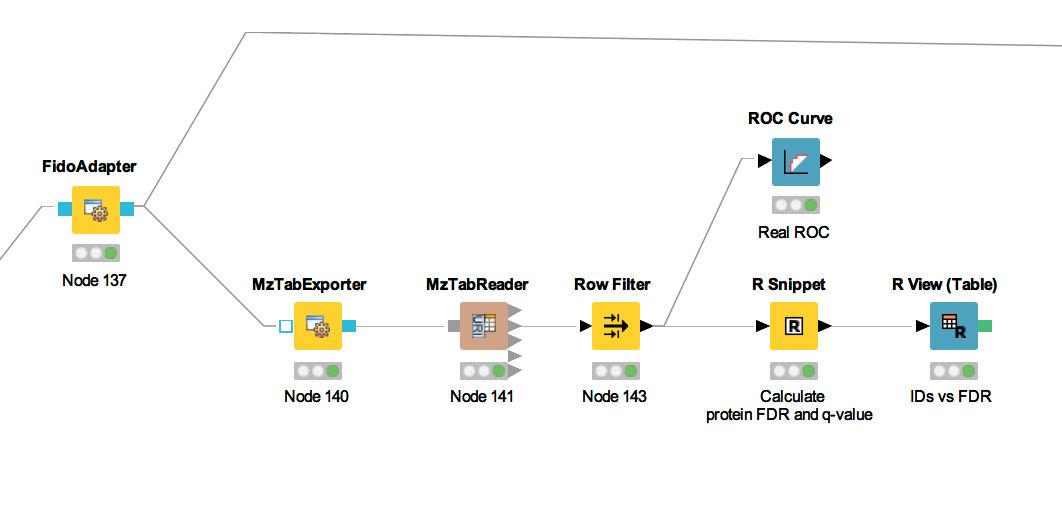
\includegraphics[width=0.85\textwidth]{graphics/protein_inference/inference_metanode.png}
  \caption{The workflow of statistical analysis of protein inference results}
  \label{fig:proteininference}
\end{figure}

\begin{figure}[htbp]
  \centering
  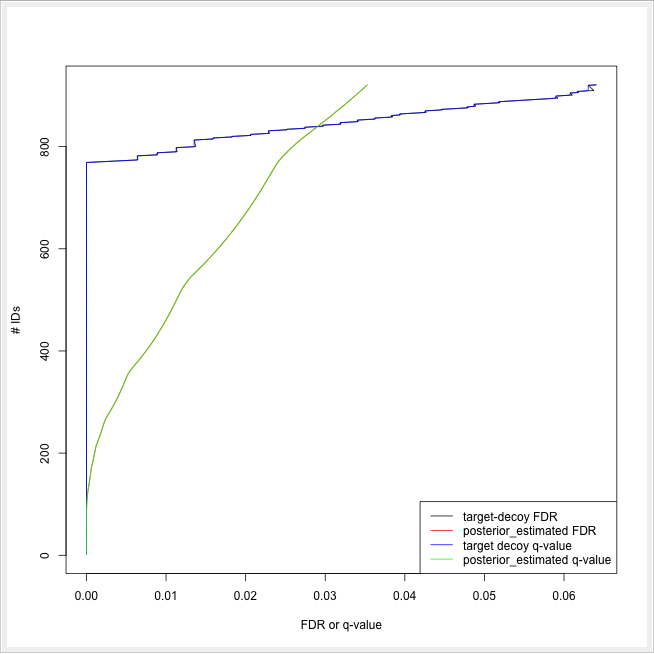
\includegraphics[width=0.45\textwidth]{graphics/protein_inference/proteinFDR.png}
  \caption{the pseudo-ROC Curve of protein IDs. The accumulated number of protein IDs is plotted on two kinds of scales: target-decoy protein FDR and Fido posterior probability estimated FDR. The largest value of posterior probability estimated FDR is already smaller than 0.04, this is because the posterior probability output from Fido is generally very high.}
  \label{fig:proteinfdr}
\end{figure}
